%%
%% PollingLab (c) 2021-24 Christopher A. Bohn
%%
%% Assignment writeup licensed under the Creative Commons Attribution 4.0 International License
%% https://creativecommons.org/licenses/by/4.0/
%%

\documentclass[12pt]{article}

\usepackage{pdflscape}
\usepackage{multicol}
\setlength{\columnsep}{2cm}
\setlength{\columnseprule}{0.4pt}
%%
%% labs/common/assignment.tex
%% (c) 2021-23 Christopher A. Bohn
%%
%% Licensed under the Apache License, Version 2.0 (the "License");
%% you may not use this file except in compliance with the License.
%% You may obtain a copy of the License at
%%     http://www.apache.org/licenses/LICENSE-2.0
%% Unless required by applicable law or agreed to in writing, software
%% distributed under the License is distributed on an "AS IS" BASIS,
%% WITHOUT WARRANTIES OR CONDITIONS OF ANY KIND, either express or implied.
%% See the License for the specific language governing permissions and
%% limitations under the License.
%%

\usepackage{addfont}
\usepackage{amsmath}
\usepackage{amssymb}
\usepackage{animate}
\usepackage{bold-extra}
\usepackage{cancel}
\usepackage{caption}
\usepackage{ccicons}
\usepackage{enumitem}
\usepackage{etoolbox}
\usepackage{fancyhdr}
\usepackage{fullpage}
\usepackage{graphicx}
\usepackage{hyperref}
\usepackage[utf8]{inputenc}
\usepackage[procnames]{listings}
%\usepackage{media9}
\usepackage{multicol}
\usepackage{subfig}
\usepackage{textcomp}
\usepackage{tikz}
\usepackage[americanresistor]{circuitikz}
%\usepackage{tikz-uml}
\usetikzlibrary{automata,positioning,arrows}
\usepackage[normalem]{ulem}
\usepackage{wrapfig}
\usepackage{xcolor}
%\usepackage[dvipsnames]{xcolor}
\definecolor{LightGreen}{rgb}{0.88,1,0.88}

\lstset{language=C, tabsize=4, upquote=true, basicstyle=\ttfamily}
\newcommand{\function}[1]{\textbf{\lstinline{#1}}}
\setlength{\headsep}{0.7cm}
\hypersetup{colorlinks=true}

%% CREDIT FOR MARKERLESSFOOTNOTE WHERE CREDIT IS DUE: https://tex.stackexchange.com/questions/30720/footnote-without-a-marker?answertab=scoredesc#tab-top
\newcommand\markerlessfootnote[1]{%
    \begingroup
    \renewcommand\thefootnote{}\footnote{#1}%
    \addtocounter{footnote}{-1}%
    \endgroup
}

\newcommand{\pagelayout}{
    \pagestyle{fancy}
    \fancyhf{}
    \lhead{\coursenumber}
    \chead{\ Lab \labnumber: \labname}
    \rhead{\courseterm}
    \cfoot{\shortlabname-\thepage}
}

\newcommand{\labidentifier}{
    \title{\ Lab \labnumber}
    \author{\labname}
    \date{Due: \duedate}
    \maketitle

    \textit{\collaborationrules}
    \markerlessfootnote{\tiny{\ifdefstring{\instructorname}{Christopher A. Bohn}{Assignment}{Original assignment} and starter code \copyright\ Christopher A. Bohn, licensed under the Creative Commons Attribution 4.0 International License~\ccby\ and under the Apache License Version 2.0, respectively.}}
    \ifdefstring{\instructorname}{Christopher A. Bohn}{}{\markerlessfootnote{\tiny{Configured for \coursenumber\ at \institutename\ by \instructorname.}}}

    \begin{description}
        \item[Obtaining the starter code] \filesource
        \item[Runtime environment] We will grade this assignment by compiling and running it on \runtimeenvironment;
            you should compile and test your code on \runtimeenvironment\ before turning it in.
        \item[Submitting your work] \filesubmission
    \end{description}
}

% display module fonts for hardware kit
% use with the Capital baseball "matrix printer" font collection (https://www.ctan.org/tex-archive/fonts/capbas/)
% Identifying the specific font in the assignment sheet is deprecated
%   -- instead, set the `usedisplayfont` boolean and the `displaymodule` variable in semester.tex,
%      and \display{...} in the assignment sheet

\addfont{OT1}{d7seg}{\dviiseg}
\addfont{OT1}{deseg}{\deseg}
\addfont{OT1}{necker}{\necker}

\providebool{usedisplayfont}

\newcommand{\display}[1]{
    \ifboolexpe{bool{usedisplayfont}}{
        \ifdefstring{\displaymodule}{MAX7219digits}{{\dviiseg #1}}{}
        \ifdefstring{\displaymodule}{MAX7219matrix}{{\deseg #1}}{}
        \ifdefstring{\displaymodule}{LCD1602}{{\necker #1}}{}
        % We don't yet have a Cow Pi configuration with 14-segment displays, so no \deseg yet
    }{
        \texttt{#1}
    }
}

\newcommand{\rubricitem}[2]{\item[\underline{\hspace{1cm}} +#1] #2}
\newcommand{\bonusitem}[2]{\item[\underline{\hspace{1cm}} Bonus +#1] #2}
\newcommand{\penaltyitem}[2]{\item[\underline{\hspace{1cm}} -#1] #2}
\newcommand{\checkoffitem}[1]{\item (\phantom{xxx}) #1}
\newcommand{\precheckoffitem}[1]{\item [] (\phantom{xxx}) #1}

\newcommand{\institutename}{University of Nebraska-Lincoln}
\newcommand{\instructorname}{Christopher A. Bohn}
\newcommand{\coursenumber}{CSCE~231}
\newcommand{\cstwo}{CSCE~156, RAIK~184H, or SOFT~161}
\newcommand{\courseterm}{Spring 2025}
\newcommand{\labnumber}{10}
\newcommand{\labname}{Using Polling with Memory-Mapped Input/Output}
\newcommand{\shortlabname}{PollingLab}
\newcommand{\duedate}{Week of April 14, before the start of your lab section}
\newcommand{\pathone}{chap09/io/memory-mapped}
\newcommand{\pathtwo}{chap09/system-descriptions/number-builder}
\newcommand{\filesource}{Download \startercode\ from Canvas, or copy \startercode\ from {\footnotesize$\sim$}cbohn2/csce231 on \textit{nuros.unl.edu}}
\newcommand{\filesubmission}{When you have completed this assignment, submit \requiredfiles\ to the assignment in Canvas.}
\newcommand{\runtimeenvironment}{a Cow Pi development board with a \processor\ microcontroller}
\newcommand{\startercode}{pollinglab.zip or pollinglab.tar}
\newcommand{\requiredfiles}{\textit{io\_functions.c} and \textit{number\_builder.c}}
\newcommand{\buildsystem}{platformio}
\newcommand{\processor}{RP2040}
\newcommand{\lowercaseprocessor}{rp2040}
\newcommand{\collaborationrules}{During your scheduled lab time, you may, \textbf{but are not required to}, form a partner group of 2 students.
    When necessary, there may be a group of 3 students.
    During your scheduled lab time, and until the end of your lab day, you may discuss problem decomposition and solution design with your lab partner.
    After your scheduled lab day, you may discuss concepts and syntax with other students, but you may discuss solutions only with the professor and the TAs.
    Sharing code with or copying code from another student or the internet is prohibited.
}
\newcommand{\policyforcodethatdoesnotcompile}{\subsection*{No Credit for Uncompilable Code}
    If the TA cannot create an executable from your code, then your code will be assumed to have no functionality.\footnote{
        At the TA's discretion, if they can make your code compile with \textit{one} edit (such as introducing a missing semicolon) then they may do so and then assess a 10\% penalty on the resulting score.
        The TA is under no obligation to do so, and you should not rely on the TA's willingness to edit your code for grading.
        If there are multiple options for a single edit that would make your code compile, there is no guarantee that the TA will select the option that would maximize your score.
    }
    Before turning in your code, be sure to compile and test your code on \runtimeenvironment\ with the original driver code, the original header file(s), and the original \textit{Makefile}.}
\newcommand{\latepolicy}{\subsection*{Late Submissions}
    This assignment is due before the start of your lab section.
     After you have exhausted your grace days, we will accept late turn-ins up to one hour late, assessing a 10\% penalty on these late submissions.
    After you have exhausted your grace days, any work turned in more than one hour late will not be graded.}
\newcommand{\softwareengineeringfrontmatter}{\section*{No Spaghetti Code Allowed}
        In the interest of keeping your code readable, you may \textit{not} use
        any \lstinline{goto} statements, nor may you use any
        \lstinline{continue} statements, nor may you use any \lstinline{break}
        statements to exit from a loop, nor may you have any functions
        \lstinline{return} from within a loop.}
\newcommand{\softwareengineeringpenalties}{\penaltyitem{1}{for each \lstinline{goto} statement,
            \lstinline{continue} statement, \lstinline{break} statement used to
            exit from a loop, or \lstinline{return} statement that occurs within
            a loop.}}
\newcommand{\scenariointroduction}{    Archie walks up to you, along with Herb Bee from Eclectic Electronics.
    Herb is holding a tangled mess of electronics.
    Archie explains, ``Herb here has developed a prototype of a device that he thinks will be useful for our physical security needs, as well as a few other applications around here. He calls it the \textit{Cow Pi}.''

    You look at the device in Herb's hands and see the Raspberry Pi Pico central to the circuit.
    ``I suppose the `\textit{-Pi}' suffix is because it uses a Raspberry Pi Pico?''
+        
    Herb replies, ``Um, yeah, sure.
 We considered using an Arduino Nano, but \textit{Cowduino} isn't very punny, is it?''

    Archie chimes in, ``Maybe with the right emphasis: \textit{Cow-DOO-ino}.''

    ``That's kind of subtle, don't you think? How will people know to put the emPHAsis on that sylLAble?''
    
    ``I think we're getting off topic here,'' you point out.
    ``How can I help?''

    ``Oh, right,'' Herb says, ``We'd like you to kick its proverbial tires.
    Let's start off with something simple, like a number builder tool.''}
\newcommand{\scenariowrapup}{Herb looks over your work.
    ``Hmm, yes. I think this is coming along nicely.
    Let's run a few more tests.''

    Archie storms into the room.
    ``We have \textit{got} to do something about security!
    How's that doodad coming along? 
    Because there's now a half-man/half-fly in the labs going on-and-on about Chaos Theory and how if we just give him a MacBook and a spaceship then he'll be able to get the Lord of Thunder to travel across the 8th Dimension.
    Is that thing just about ready?''

    Herb shakes his head, ``No, not quite yet. It should be ready in about a week.''}


\lstset{language=c, numbers=left, showstringspaces=false,
    moredelim = [s][\ttfamily]{/*}{*/} % I shouldn't need this parameter!
}

\pagelayout
\begin{document}
    \labidentifier\

    \pdfbookmark[1]{Frontmatter}{frontmatter}                                       The purpose of this assignment is to give you more confidence in C programming
and to begin your exposure to the underlying bit-level representation of data.

The instructions are written assuming you will edit and run the code on
\runtimeenvironment. If you wish, you may edit and run the code
in a different environment; be sure that your compiler suppresses no warnings,
and that if you are using an IDE that it is configured for C and not C++.

\section*{Learning Objectives}

After successful completion of this assignment, students will be able to:
\begin{itemize}
    \item Use the ASCII table to determine the corresponding integer values of C
    \lstinline{char} values.
    \item Apply arithmetic operators and comparators to C \lstinline{}{char} values.
    \item Construct and use a bitmask.
    \item Use bitwise operators and bit shift operators to create and modify values.
\end{itemize}

\subsection*{Continuing Forward}

Your experience with viewing values as bit patterns will be applicable in
future labs, as will bit masks and bit operations. Some of the functions you
write in this lab will be used in the next lab.

\section*{During Lab Time}

During your lab period, the TAs will demonstrate how to read the ASCII table and
will provide a refresher on bitwise AND, bitwise OR, and left- and right-shifts.
During the remaining time, the TAs will be available to answer questions.

Before leaving lab, \textit{at a minimum} \dots


    \softwareengineeringfrontmatter

    \section*{Scenario}                                                             \scenariointroduction

    \section{Assignment Summary}                                                    Please familiarize yourself with the entire assignment before beginning.
There are three parts to this assignment.

\subsection{Why are There Letters on Telephone Keypads?}

Once upon a time, telephone exchanges were staffed by operators who would use patch cords on a switchboard to connect callers.
If you needed to make a local-area call to someone whose phone was serviced by a different exchange, then you needed to tell your operator which exchange to connect to.
Letters were assigned to digits so that easy-to-remember -- and audibly-distinctive -- mnemonics could be formed such that the first two letters of the mnemonic that correspond to the 2-digit exchange identifier.
For example, the 86 exchange would use a mnemonic that started with a `T', `U', or `V' and that has as a second letter an `M', `N', or `O' --
so 867--5309 might be ``University 7--5309''.

The presence of letters on telephone dials and (later) telephone keypads allowed for custom phone numbers that used words formed by the available letters.
For example, a bank's phone number might be 472--2265, aka 472--BANK.
Less fictionally, 1--800--FLOWERS was used by a company that partnered with florists to allow people to have bouquets delivered anywhere in the U.S\@.

When the Short Message Service protocol was introduced to allow text-based communication by taking advantage of unused bytes in the handshake between cellular phones and the cell network, naturally the letters that were already present on the keypad were used to tap out messages.

While QWERTY keyboards on smartphones have largely replaced the 10-digit keypad for text entry, the letters remain, waiting for the next clever use\dots

\subsection{Constraints} \label{subsec:constraints}

You may \textit{not} poll the matrix keypad nor the pushbuttons to determine if they have been pressed.
You must use interrupts to determine if a key or button has been pressed.
Once an interrupt has fired, you may scan the matrix keypad or read the pushbuttons to determine which key has been pressed or whether the button has been pressed or released.

You may use any features that are part of the C standard if they are supported by the compiler.
You may use the constants and functions provided in the starter code.

\subsubsection{Constraints on the Arduino core}

You may \textit{not} use any libraries, functions, macros, types, or constants from the Arduino core.

%\subsubsection{Constraints on AVR-libc}
%
%You may use any AVR-specific functions, macros, types, or constants of avr-libc.\footnote{
%    \url{https://www.nongnu.org/avr-libc/user-manual/index.html}
%}

\ifdefstring{\processor}{ATmega328P}{
    \subsubsection{Constraints on AVR-libc}

    You may not use any AVR-specific functions, macros, types, or constants of avr-libc.\footnote{\url{https://www.nongnu.org/avr-libc/user-manual/index.html}}
}{}
\ifdefstring{\processor}{RP2040}{
% TODO: parameterize this (when we eventually port to the bare-metal Arduino toolchain, and to the Pico SDK)
    \subsubsection{Constraints on MBED OS}

    You may not use any functions, macros, types or constants from MBED that are not part of the C standard.\footnote{\url{https://os.mbed.com/docs/mbed-os/v6.16/introduction/index.html}}
}{}

\subsubsection{Constraints on the CowPi library}

You may use any functions provided by the CowPi\footnote{
    \url{https://cow-pi.readthedocs.io/en/latest/library.html}
}
and the CowPi\_stdio\footnote{
    \url{https://cow-pi.readthedocs.io/en/latest/stdio.html}
} libraries,
and you may use any data structures\footnote{
    \url{https://cow-pi.readthedocs.io/en/latest/microcontroller.html}
} provided by the CowPi library.

\subsubsection{Constraints on other libraries}

You may \textit{not} use any libraries beyond those explicitly identified here.


    \section{Getting Started}                                                       Download the zip file or tarball from \filesource.
Once downloaded, unpackage the file and open the project in your IDE\@.

\subsection{Description of RangeFinder Files}

\subsubsection{combolock.c, interrupt\_support.h, interrupt\_support.cpp, display.h, display.cpp}

Do not edit \textit{combolock.c}, \textit{interrupt\_support.h}, \textit{interrupt\_support.cpp}, \textit{display.}, or \textit{display.cpp}.

These files contain code to simplify interrupt management, and functions to place text on the display module.

\subsubsection{rotary-encoder.h \& rotary-encoder.c}

Do not edit \textit{rotary-encoder.h}

The \textit{rotary-encoder.c} file is where you will process inputs from the rotary encoder.

\subsubsection{servomotor.h \& servomotor.c}

Do not edit \textit{servomotor.h}

The \textit{servomotor.c} file is where you will control the servomotor.

\subsection{lock-controller.h \& lock-controller.c}

Do not edit \textit{lock-controller.h}

The \textit{lock-controller.c} file is where you will implement the logic for the combination lock.

%\subsubsection{shared\_variables.h}
%
%The \textit{shared\_variables.h} header file is where you will place any types that you define and where you will externalize any global variables that need to be used by more than one \textit{.c} file.
%
%It also contains a structure that you may use to access an analog-digital converter's registers,
%and it contains meaningfully-named constants to refer to specific pins you will use in this assignment.


\subsection{Assemble the Hardware}

\textcolor{red}{\textbf{BEFORE YOU PROCEED FURTHER:}}
\begin{description}
    \checkoffitem{Add the new hardware to your Cow~Pi as described in Appendix~\ref{sec:hardwareMods-mk4b}.}
\end{description}


    \section{Initial Changes to the Code} \label{sec:LabTime}                       During your lab period, the TAs will guide the class through the first modifications to the starter code that you must make, described in this section.
If you do not attend your lab period, then you must complete this section on your own.
\textbf{\textit{Except during lab time, you may }not\textit{ discuss the solutions for this section with other students.}}




\subsection{Populate the Keypad's Lookup Table} \label{subsec:populatekeypad}

Locate the \lstinline{keys} $4 \times 4$ nested array on lines 34--39 of \textit{io\_functions.c}.
This nested array serves as a lookup table to obtain the appropriate value when a key is pressed.
\textit{Even the starter code depends on this nested array being populated correctly.}
The element \lstinline{keys[0][0]} will correspond to the \texttt{1} key;
\lstinline{keys[0][3]} will correspond to the \texttt{A} key;
\lstinline{keys[3][0]} will correspond to the \texttt{*} key;
and \lstinline{keys[3][3]} will correspond to the \texttt{D} key.

We want the numerals \texttt{0}--\texttt{9} to produce their respective decimal (and hexadecimal) values.
We want \texttt{A}--\texttt{D} to produce their respective hexadecimal values.
We want \texttt{\#} to produce the hexadecimal value 0xE, and we want \texttt{*} to produce the hexadecimal value 0xF\@.

\begin{description}
    \checkoffitem{Populate \lstinline{keys}' nested array initializer so that the lookup table will produce the correct value for each row/column combination.}
\end{description}

\subsubsection*{Test your code}

You can confirm that you correctly populated the array's initializer by running the test code.
\begin{description}
    \checkoffitem{Place the \textbf{left switch} in the \textit{right} position and the \textbf{right switch} in the \textit{left} position, and upload your code.
        (Or, if you have already uploaded your code, position the switches and press the RESET button.)}
\end{description}
The test code will output on the display module.
The output will include the key that was pressed (if any), a hyphen if no key is being pressed, or a question mark if \function{get_keypress()} returns an invalid value.

\newcommand{\firstline}{1}

\ifdefstring{\processor}{ATmega328P}{\renewcommand{\firstline}{346}}{}
\ifdefstring{\processor}{RP2040}{\renewcommand{\firstline}{345}}{}
\begin{lstlisting}[numberstyle=\color{gray}, numbers=left, firstnumber=\firstline, basicstyle=\ttfamily\small]
...
if (key_pressed <= 0x0F) {
    sprintf(output, ''%2X%5c%2c%4c%2c'',
            key_pressed,
            left_button_position ? 'D' : 'U', right_button_position ? 'D' : 'U',
            left_switch_position ? 'R' : 'L', right_switch_position ? 'R' : 'L');
}  else {
    sprintf(output, ''%2c%5c%2c%4c%2c'',
            key_pressed == 0xFF ? '-' : '?',
            left_button_position ? 'D' : 'U', right_button_position ? 'D' : 'U',
            left_switch_position ? 'R' : 'L', right_switch_position ? 'R' : 'L');
}
...
\end{lstlisting}
%...
%if (key_pressed <= 0x0F) {
%    sprintf(output, "%2X%5c%2c%4c%2c",
%    key_pressed,
%    left_button_position ? 'D' : 'U', right_button_position ? 'D' : 'U',
%    left_switch_position ? 'R' : 'L', right_switch_position ? 'R' : 'L');
%}  else {
%    sprintf(output, "%2c%5c%2c%4c%2c",
%    key_pressed == 0xFF ? '-' : '?',
%    left_button_position ? 'D' : 'U', right_button_position ? 'D' : 'U',
%    left_switch_position ? 'R' : 'L', right_switch_position ? 'R' : 'L');
%}
%...

Familiarize yourself with the test code's other outputs.
The output will include the positions of the left and right buttons (``U'' for up and ``D'' for down) and of the left and right switches (``L'' for left position and ``R'' for right position).

Finally, if both buttons are pressed then the left LED will illuminate, and if both switches are in the right position then the right LED will illuminate.

\ifdefstring{\processor}{ATmega328P}{\renewcommand{\firstline}{326}}{}
\ifdefstring{\processor}{RP2040}{\renewcommand{\firstline}{325}}{}
\begin{lstlisting}[numberstyle=\color{gray}, numbers=left, firstnumber=\firstline]
    ...
    set_left_led(left_button_position && right_button_position);
    set_right_led(left_switch_position && right_switch_position);
    ...
\end{lstlisting}


\subsection{Determine the Base Addresses of Certain I/O Register Banks} \label{subsec:baseAddresses}

In Sections~\ref{subsec:detectKeyAction}--\ref{subsec:controlLED} and \ref{subsec:simpleIO}--\ref{subsec:ScannedInput}, you will use
\ifdefstring{\processor}{ATmega328P}{an array of \lstinline{cowpi_ioport_t} structures}{}
\ifdefstring{\processor}{RP2040}{a \lstinline{cowpi_ioport_t} structure}{}
to access the memory-mapped I/O registers for the \processor's data pins.

In Section~\ref{subsec:timer}, you will use a pointer to a
\ifdefstring{\processor}{ATmega328P}{\lstinline{cowpi_timer8bit_t}}{}
\ifdefstring{\processor}{RP2040}{\lstinline{cowpi_timer_t}}{}
structure to determine how much time has elapsed since the system was powered-up.

Read the section of the Cow~Pi datasheet that \href{https://cow-pi.readthedocs.io/en/latest/CowPi_\lowercaseprocessor/io_registers.html#structure-for-memory-mapped-input-output}{discusses the \lstinline{cowpi_ioport_t} structure}.
(During the guided discussion in your lab period, the TAs may direct you to particular parts of that section of the datasheet,
but be sure to go back and read the full section covering \href{https://cow-pi.readthedocs.io/en/latest/CowPi_\lowercaseprocessor/io_registers.html#external-pins-input-output}{input/output pins} later.)
After you have done so,
\begin{description}
    \checkoffitem{Uncomment the
        \ifdefstring{\processor}{ATmega328P}{\lstinline{ioports = ...}}{}
        \ifdefstring{\processor}{RP2040}{\lstinline{ioport = ...}}{}
        line of the starter code's \function{initialize_io()} function, and}
    \checkoffitem{Assign the appropriate address to the
        \ifdefstring{\processor}{ATmega328P}{\lstinline{ioports = ...}}{}
        \ifdefstring{\processor}{RP2040}{\lstinline{ioport = ...}}{}
        pointer on that line.}
\end{description}

\input{../../../\pathone/assignment/initialize_io-\lowercaseprocessor}

You can now use the
\ifdefstring{\processor}{ATmega328P}{
    \lstinline{ioports} pointer as an array of \lstinline{cowpi_ioport_t} structures, which you can index using the \lstinline{D0_D7}, \lstinline{D8_D13}, and \lstinline{D14_D19} named constants.
}{}
\ifdefstring{\processor}{RP2040}{\lstinline{ioport} pointer to access the microcontroller pins' inputs and outputs.}{}


Read the section of the Cow~Pi datasheet that \href{https://cow-pi.readthedocs.io/en/latest/CowPi_\lowercaseprocessor/io_registers.html#timers}{discusses the timer registers}.
\ifdefstring{\processor}{ATmega328P}{
    Pay attention to the \lstinline{cowpi_timer8bit_t} structure and to TIMER0's registers.
}{}
After you have done so,
\begin{description}
    \checkoffitem{Uncomment the \lstinline{timer = ...} line of the starter code's \function{initialize_io()} function, and}
    \checkoffitem{Assign the appropriate address to the \lstinline{timer} pointer on that line.}
\end{description}

When you get to the assignment's Section~\ref{subsec:timer}, you will be able to use the \lstinline{timer} pointer to access the timer's memory-mapped registers to read its counter.


\subsection{Detect Whether a Key on the Numeric Keypad Has Been Pressed} \label{subsec:detectKeyAction}

The next part of the group activity is detecting when someone is pressing a key on the numeric keypad.
The \function{key_is_pressed()} function in the starter code is:

\input{../../../\pathone/assignment/key_is_pressed-\lowercaseprocessor}

Line~\ref{code:readColumns} uses the Arduino function \function{digitalRead()} to read the values on the four pins attached to the keypad's columns.
If any of those pins has a 0 on it, then a key has been pressed (see Section~\ref{subsec:ScannedInput}).
The next line debounces that reading (see Section~\ref{subsec:debouncing}).

%The remainder of the code compares the reading to the previous reading.
%If no key was pressed and there is still no key being pressed, the function returns \lstinline{false}.
%Similarly, if a key was pressed and is still being pressed, the function returns \lstinline{false}.
%On the other hand, if no key was pressed and there is now a key being pressed, or if a key was being pressed and there is now no key being pressed, then the function returns \lstinline{true}.

One problem is that the \function{digitalRead()} function is part of the Arduino core and, as noted in Section~\ref{subsec:constraints}, you may not use functions from the Arduino core.
The other problem is that the \function{digitalRead()} function can read only one pin at a time, and so there are four distinct reads.
Now that you have the base address for the
\ifdefstring{\processor}{ATmega328P}{\lstinline{ioports} array,}{}
\ifdefstring{\processor}{RP2040}{\lstinline{ioport} structure,}{}
you can use memory-mapped I/O to replace the calls to \function{digitalRead()},
and you can do so in a manner that obtains the values on all four pins at the same time.

\ifdefstring{\processor}{ATmega328P}{
    \newcommand{\mappingtablelink}{id9}
    \newcommand{\mappingtablenumber}{8}
}{}
\ifdefstring{\processor}{RP2040}{
    \newcommand{\mappingtablelink}{id16}
    \newcommand{\mappingtablenumber}{22}
}{}
If you are currently in your lab period, then work with the other students in your lab section to determine the answers to these questions.
If you are not attending your lab period, then work individually to determine the answers to these questions.
\begin{description}
    \checkoffitem{Using the datasheet's} \href{https://cow-pi.readthedocs.io/en/latest/CowPi_\lowercaseprocessor/io_registers.html#\mappingtablelink}{Table~\mappingtablenumber}:
        \begin{itemize}
            \ifdefstring{\processor}{ATmega328P}{
                \item What should you use to index the \lstinline{ioports} array to read from pins~14--17, the pins connected to the keypad's columns?
                \item What field in that element should you use?
            }{}
            \item What bitmask should you use?
            \item What should line~\ref{code:readColumns} look like?
        \end{itemize}
    \checkoffitem{Replace line~\ref{code:readColumns} with code that reads from a memory-mapped input register to determine whether a key is being pressed.}
\end{description}



\subsubsection*{Test your code}

You can confirm that you correctly detected a change on the keypad by running the test code.
\begin{description}
    \checkoffitem{Place the both switches in the \textit{right} position and upload your code.
        (Or, if you have already uploaded your code, position the switches and press the RESET button.}
\end{description}
The test code will output on the display module.
The output will indicate whether a key is being pressed, and also the elapsed time since the system was powered up.


\subsection{Controlling an LED} \label{subsec:controlLED}

The final part of the group activity is illuminating and deluminating the built-in LED\@.
Locate the \function{set_left_led()} function.
In the starter code, this function is implemented by calling functions in the CowPi library.

\begin{description}
    \checkoffitem{Modify this function to replace the calls to CowPi library functions with code that uses the
    \ifdefstring{\processor}{ATmega328P}{\lstinline{ioports} array,}{}
    \ifdefstring{\processor}{RP2040}{\lstinline{ioport} pointer,}{}
    to turn the LEDs on or off.}
        \begin{description}
            \checkoffitem{Use the read-modify-write pattern to do so, so that you do not change any pins that you do not intend to change.\footnote{Even on ``input'' pins, changing the ``output'' register can have an effect.}}
                \begin{itemize}
                    \ifdefstring{\processor}{ATmega328P}{
                        \item What should you use to index the \lstinline{ioports} array to access the pin connected to that LED?
                        What field in that element should you use?
                    }{}
                    \ifdefstring{\processor}{RP2040}{
                        \item Which field in the \lstinline{cowpi_ioport_t} structure should you use?
                    }{}
                    \item When turning the LED on, what bitmask should you use?
                    What operation should you use?
                    \item When turning the LED off, what bitmask should you use?
                    What operation should you use?
                \end{itemize}
            \item[\phantom{xxx}$\bullet$] No debouncing code is necessary because these functions do not read from mechanical switches.
        \end{description}
\end{description}

\paragraph{Test your code}

\begin{description}
    \checkoffitem{Place the \textbf{left switch} in the \textit{right position} and upload the program to your Cow~Pi.}
\end{description}
Whenever both buttons are pressed, the left LED will illuminate.


\vspace{1cm}

You are now ready to complete the remainder of this assignment on your own.
Reminders:
\begin{itemize}
    \item You can complete Sections~\ref{sec:MemMapIO} and \ref{sec:SimpleSystem} in either order.
    \item \collaborationrules
\end{itemize}


    \section{Memory-Mapped Input/Output} \label{sec:MemMapIO}                       In this section, you will use the data structures provided by the CowPi library to access the \developmentboard's memory-mapped I/O registers.
All functions that you edit in this part of the assignment are in \textit{io\_functions.c}
You will use the same test code from Section~\ref{sec:GettingStarted} to test your code.

\textit{Remember that to start the I/O test code, the \textbf{left switch} must be in the \underline{right} position when the \developmentboard\ restarts.}

You can complete this part of the assignment before or after implementing the system from Section~\ref{sec:SimpleSystem}.
You must, however, complete Section~\ref{sec:LabTime} first.
If you have already implemented the system from Section~\ref{sec:SimpleSystem}, you may want to make a backup copy of your program now.


\subsection{Simple Inputs and Outputs} \label{subsec:simpleIO}

Because you have already completed Section~\ref{sec:LabTime}, you can use the \lstinline{ioports} pointer as an array of \lstinline{cowpi_ioport_t} structures, which you can index using the \lstinline{D0_D7}, \lstinline{D8_D13}, and \lstinline{D14_D19} named constants.
Use the \lstinline{.input} field with bitmasks to read inputs.
Use the \lstinline{.output} field with bitmasks and the read-modify-write pattern to write outputs.
During lab, the TAs covered reading from inputs and using the read-modify-write pattern to write outputs;
however, if you missed lab or have forgotten, you can find examples in Section~4.1.1 of the Cow Pi datasheet.

\subsubsection{Simple Inputs}

Locate the \function{left_button_is_pressed()}, \function{right_button_is_pressed()}, \\ \function{left_switch_in_right_position()}, and  \function{right_switch_in_right_position()} functions.
In the starter code, these functions are implemented by calling functions in the CowPi library.

\begin{itemize}
    \item Replace the calls to CowPi library functions with code that uses the \lstinline{ioports} array to ascertain the controls' positions.
    \item Do \textit{not} remove the calls to \function{debounce_byte()}!
\end{itemize}

\paragraph{Test your code}

Place the left switch in the right position and upload the program to your \developmentboard.
The output will include the positions of the left and right buttons (``U'' for up and ``D'' for down) and of the left and right switches (``L'' for left position and ``R'' for right position).


\subsubsection{Simple Outputs}

Locate the \function{set_left_led()} and \function{set_right_led()} functions.
In the starter code, these functions are implemented by calling functions in the CowPi library.

\begin{itemize}
    \item Modify these two functions to replace the calls to CowPi library functions with code that uses the \lstinline{ioports} array to turn the LEDs on or off.
    \item Use the read-modify-write pattern to do so, so that you do not change any pins that you do not intend to change.\footnote{Even on ``input'' pins, changing the ``output'' register has an effect.}
    \item No debouncing code is necessary because these functions do not read from mechanical switches.
\end{itemize}

\paragraph{Test your code}

Place the left switch in the right position and upload the program to your \developmentboard.
If both buttons are pressed then the left LED will illuminate, and if both switches are in the right position then the right LED will illuminate.

\vspace{1cm}

This would be a good time to make a backup copy of your program.


\subsection{Scanned Input} \label{subsec:ScannedInput}

Locate the \function{get_keypress()} function.
The implementation in the starter code determines whether there has been a change on the keypad.
If so, it calls the CowPi library's \function{cowpi_get_keypress()} function.
The \function{cowpi_get_keypress()} function returns a \lstinline{char} corresponding to the character on the pressed key,
but the \function{get_keypress()} function is supposed to return a \lstinline{uint8_t} that has the hexadecimal value of the pressed key (considering \# as 0xE and * as 0xF).
Because of this, the rest of the implementation is a \lstinline{switch} statement to obtain the correct value from the \function{keys} nested array.

Read Section~1.2 of the Cow Pi datasheet.
After you have done so:

\begin{itemize}
    \item Preserve the debouncing code in \function{get_keypress()}, and
    \item Replace the starter code's call to \function{cowpi_get_keypress()} and \lstinline{switch} statement with code that scans the keyboard.
        \begin{itemize}
            \item Use the \lstinline{ioports} array to read from and write to the appropriate pins,
            \item Use \lstinline{delayMicroseconds(1)} for the delay shown on line 4 of the pseudocode in Section~1.2.2 of the datasheet, and
            \item Use the \lstinline{keys} nested array to obtain the correct integer value for the key at a given row and column.
        \end{itemize}
\end{itemize}

\ifbool{offerdecompositionhints}{
    \subsubsection*{Suggestions}
    Look at the pseudocode in the datasheet's Section~1.2.2 and relate it to the ``theory of operation'' in the datasheet's Section~1.2.1.
    Even though the pseudocode is expressed as nested loops, you do not need to implement it that way.
    We have seen implementations that have an outer loop for the rows and an inner loop for the columns,
    and we have seen implementations that have a loop for the rows but use a \lstinline{switch} statement or chained \lstinline{if} statements to enumerate the possibilities for the columns.
    With four rows and four columns, both are viable solutions.

    The key insights are:
    \begin{itemize}
        \item Each of the row vectors you output will have exactly one ``0'' bit;
            the placement of that ``0'' corresponds to exactly one of the rows in the \lstinline{keys} nested array, and
        \item Each of the column vectors you read as input, if it is not 0xF, will have exactly one ``0'' bit;
            the placement of that ``0'' corresponds to exactly one of the columns in the \lstinline{keys} nested array
    \end{itemize}

    Even though you \textit{can} set the loop conditions to terminate the loop as soon as the pressed key has been determined,\footnote{
        I am \textit{not} saying you can \lstinline{return} from inside the loop or \lstinline{break} out of the loop;
        I am saying you can write a \lstinline{while} condition that includes testing whether \lstinline{key_pressed} is still 0xFF.
    } it would be better to keep your loop conditions simple and allow the code to examine all sixteen keys.
    With only sixteen keys, there isn't much time savings to be had by ending the loop as soon as the key has been found,
    and in a ``real'' embedded system, our time budget would have to allow enough time to examine all sixteen keys and so any ``savings'' gained by ending the loop early would be lost to sitting idle later.
}{}

\subsubsection*{Test your code}

Place the left switch in the right position and upload the program to your \developmentboard.
The output will include the key that was pressed (if any), a hyphen if no key is being pressed, or a question mark if \function{get_keypress()} returns an invalid value.

\vspace{1cm}

This would be a good time to make a backup copy of your program.


\subsection{Display Module} \label{subsec:DisplayModule}

You will use a pointer to a \lstinline{cowpi_i2c_t} structure to access the memory-mapped I/O registers for the \developmentboard's I$^2$C (aka ``TWI'') hardware,
and you will use those registers to send data to the display module.

Read Section~1.3 of the Cow Pi datasheet to familiarize yourself with the physical characteristics of the display module.
Read the datasheet's Section~4.2 to familiarize yourself with the I$^2$C registers (Sections~4.2.1--4.2.2), with the I$^2$C handshake and transmission sequence (Section~4.2.3), and with the data format and the steps required by the display module itself (Section~4.2.4). After you have done so:

\begin{itemize}
    \item Uncomment the second line of the starter code's \function{initialize_io()} function, and
    \item Assign the appropriate address to the \lstinline{i2c} pointer on that line.
\end{itemize}

You can now use the \lstinline{i2c} pointer to operate the I$^2$C hardware.
Now locate the \function{send_halfbyte()} function.

\begin{itemize}
    \item Implement the pseudocode from the datasheet's Section~4.2.3, to
    \item Send the three bytes of data described in the datasheet's Section~4.2.4.
        \begin{itemize}
            % \item You may handle the error conditions show in the pseudocode in whatever manner you see fit; it would be best to do so in a manner that allows you to determine \textit{which} error is occurring.
            \item Use \lstinline{delayMicroseconds(1)} to implement the pulse described in Section~4.2.4 of the datasheet.
        \end{itemize}
\end{itemize}

After you are satisfied that you have implemented the \function{send_halfbyte()} function correctly:

\begin{itemize}
    \item Uncomment the last line of the starter code's \function{initialize_io()} function to register \function{send_halfbyte()} with the CowPi library's LCD1602 code.
\end{itemize}

All of the functions in the CowPi library that send characters or commands to the display module will now make use of your \function{send_halfbyte()} function.

\ifbool{offerdecompositionhints}{
    \subsubsection*{Suggestions}
    Altogether, you will make six transmissions in the \function{send_halfbyte()} function: the start bit, the serial adapter's address, three bytes meant for the display module itself, and the stop bit.
    The start and stop bits don't have data associated with them, but the other four transmissions do.
    After each transmission (except the stop bit), you need to wait until the transmission is complete before initiating the next transmission;
    you can achieve this with a \textit{busy wait}.
    As discussed in lecture, a busy wait is simply a do-nothing loop that blocks the program while some condition holds.

    The bit vector created in line~6 of the the pseudocode in the datasheet's Section~4.2.3 consists of bits that must be set to 1 in the control register for all of these transmissions.
    When transmitting the start and stop bits, the relevant bit is also set to 1 in the control register (pseudocode line~9 and 29).
    Otherwise, only the basic bit vector is written to the control register.

    The first datum to transmit after the start bit is the serial adapter's address (properly shifted) so that the adapter knows the remaining transmissions are meant for it.
    The serial adapter will pass the data all transmissions to the display module until it receives the stop bit.
    Even though the pseudocode characterizes those transmissions as a loop over the data maent for the display module, it will be easier to implement sequentially.
    Two of the three bytes meant for the display module are identical, and the remaining byte differs only only in one bit.
    The first ensures the halfbyte, backlight, read/write, and command bits are at their correct values before a latching pulse starts.
    The second maintains those values and creates the latching pulse; a \function{delayMicroseconds()} call holds the pulse.
    Finally, the third byte ensures those values are still present as the latching pulse ends.

    \vspace{0.5cm}

    There are two aspects to this task that some students found frustrating in the past:
    \begin{itemize}
        \item Some of the required bitshifts may seem like make-work -- for example, line~16 of the pseudocode shifts the serial adapter's address to the left by one bit, but after that the least significant bit is always 0
            \begin{itemize}
                \item These bits that are seemingly constant appear so only because this assignment uses one specific part of a very flexible protocol
                \item In other uses of the I$^2$C protocol, the bits that are constant \textit{in this assignment} serve other purposes
            \end{itemize}
        \item If some part of your implementation has a bug, you aren't provided with much data you can use to form hypotheses during debugging
            \begin{itemize}
                \item ``Not much data'' is not the same as ``no data''
                    \begin{itemize}
                        \item If a busy-wait doesn't terminate, the problem is probably with your implementation of the I$^2$C protocol -- double-check the bit vectors placed in the control register, and possibly the bit vector placed in the data register when you transmit the serial adapter's address
                        \item If the function terminates but the display module doesn't update, the problem is probably with the bit vectors placed in the data register that the serial adapter will pass along to the display module, or with the ``latch'' pulse
                    \end{itemize}
                \item You can always get help from the professor or a TA with any aspect of this assignment, and you can discuss \textit{concepts and syntax} with other students;
                    \textit{without showing other students your code}, asking other students questions like these, and answering them, is acceptable:
                    \begin{itemize}
                        \item ``The datasheet says we want a `1' in bit 7, a `1' in bit 2, and `0's in the other bits; that looks like this, right?'' and then write a binary or hexadecimal bit vector on paper or a whiteboard
                        \item ``The datasheet says to shift a `1' seven places to the left, and then shift a `1' two places to the left, and then take those two results and bitwise-OR them together; would you help me remember how to do a left-shift?''
                    \end{itemize}
            \end{itemize}
    \end{itemize}
}{}

\subsubsection*{Test your code}

Place the left switch in the right position and upload the program to your \developmentboard.
If the test code displays its outputs on the display module, then you implemented \function{send_halfbyte()} correctly.
If the test code displays its outputs on the Serial Monitor but not the display module, or if the test code does not run at all, then there is an error in your code.

\vspace{1cm}

If you decide to work on other parts of the assignment before finishing \function{send_halfbyte()} then comment-out the call to \function{cowpi_lcd1602_set_send_halfbyte_function()} in \function{initialize_io()}.


    \section {Implementing a Simple System Using Polling} \label{sec:SimpleSystem}  In this section you will implement a ``number building tool'' that turns a sequence of inputs into a number.
A notional use of this number builder would be to create the operands for a calculator.
Section~\ref{subsec:functionalspecification} has the tool's specification.
You should design your system using the I/O functions in \textit{io\_functions.c} -- either the implementations from the starter code, or the implementations you wrote (or will write) from Section~\ref{sec:MemMapIO}.
All logic for your ``number building tool'' should go in \textit{number\_builder.c}.
After the specification are a few suggestions for making good use of those functions.

\textit{Remember that to start your simple embedded system, the \textbf{left switch} must be in the \underline{left} position when the \developmentboard\ restarts.}

You can complete this part of the assignment before or after implementing the I/O code from Section~\ref{sec:MemMapIO}.
You must, however, complete Section~\ref{subsec:populatekeypad} first.
If you have already implemented the I/O code from Section~\ref{sec:MemMapIO}, you may want to make a backup copy of your program now.


\subsection{Number Builder Specification} \label{subsec:functionalspecification}

%! suppress = LabelConvention
\begin{enumerate}
    \item The tool shall have two alignment modes, \textit{left justified mode} and \textit{right justified mode}. The \textbf{left switch} controls the alignment mode.
        When the \textbf{left switch} is toggled to the left, the tool shall be in left justified mode.
        When the \textbf{left switch} is toggled to the right, the tool shall be in right justified mode.
    \item If the user toggles the \textbf{left switch} (\textit{i.e.}, changes alignment mode):
        if no number is being displayed, then the system shall seamlessly transition between alignment modes;
        otherwise, the system's behavior is undefined.
    \item The tool shall have two number bases, \textit{decimal} and \textit{hexadecimal}.
        While the number shall be displayed in both number bases (requirement~\ref{spec:displayFormat}),
        the \textbf{right switch} controls which number base is used to build the number.
    \item \label{spec:decimalExplained} When the \textbf{right switch} is toggled to the left, the number builder will use the decimal number base for inputs.
        When the user presses a button on the \textbf{matrix keypad} with a decimal numeral (\textit{0-9}) then the number builder shall take the appropriate action as specified in requirement~\ref{spec:initialKeyPress} or \ref{spec:BuildingValue}.
        Any other buttons on the keypad shall be ignored.
    \item \label{spec:hexadecimalExplained} When the \textbf{right switch} is toggled to the right, the number builder will use the hexadecimal number base for inputs.
        When the user presses a button on the \textbf{matrix keypad} then the number builder shall take the appropriate action as specified in requirement~\ref{spec:initialKeyPress} or \ref{spec:BuildingValue}.
        Buttons with decimal numerals (\textit{0-9}) or alphabetic letters (\textit{A-D}) shall be interpreted as having the corresponding hexadecimal numeral;
        the button with the octothorp (\#) shall be interpreted as having the hexadecimal numeral \textit{E};
        and the button with the asterisk (*) shall be interpreted as having the hexadecimal numeral \textit{F}.
    \item If the user toggles the \textbf{right switch} (\textit{i.e.}, changes the number base):
        if no number is displayed, or if the number 0 is displayed, then the system shall seamlessly transition between number bases;
        if a non-zero number is being built then the system's behavior is undefined.
    \item Initially, the \textbf{display module} shall be blank.
    \item \label{spec:displayFormat} When the \textbf{display module} is non-blank (\textit{i.e.}, a number is being built):
        the number's decimal representation shall be on the \textbf{display module}'s top row,
        and the number's hexadecimal representation shall be on the \textbf{display module}'s bottom row.
        These representations shall be aligned to the left side or to the right side of the \textbf{display module}, in accordance with the tool's alignment mode.
    \item \label{spec:illuminateLED} Whenever the user presses a key on the \textbf{matrix keypad}, the \textbf{right LED} (aka, the external LED) shall illuminate for approximately one-half of a second.
        Whenever the user presses one of the \textbf{pushbuttons}, the \textbf{left LED} (aka the internal LED) shall illuminate for approximately one-half of a second.
    \item \label{spec:LEDoffWhenOtherwise} The \textbf{LEDs} shall not illuminate except as specified in requirement~\ref{spec:illuminateLED}.
        %Exception: the \textbf{left LED} may blink as a consequence of its pin being used as the SPI \texttt{SCK} signal.
        There is no prohibition against the \developmentboard's \texttt{TX}, \texttt{RX}, and \texttt{PWR} LEDs illuminating.
    \item The system shall build numbers in response to user input:
        \begin{enumerate}
        \item \label{spec:32bits} The numbers' values shall be representable as 32-bit signed integers.
        \item \label{spec:initialKeyPress} If the display is blank (\textit{i.e.}, there is not yet a number being built), then whenever the user presses a button on the \textbf{matrix keypad}, the corresponding numeral shall be displayed on the \textbf{display module}, either in the far-left column or the far-right column, depending on the alignment mode.
            If decimal input mode is used, then both the decimal and hexadecimal representations shall display the numeral.
            If hexadecimal input mode is used, then the hexadecimal representation shall display the numeral,
            and the decimal representation shall display the corresponding decimal value.
            The numeral displayed shall follow the interpretations specified in requirements~\ref{spec:decimalExplained} and \ref{spec:hexadecimalExplained}.
            \begin{itemize}
                \item \textit{Note:} In accordance with requirement~\ref{spec:displayFormat}, the number shall be displayed in both decimal and in hexadecimal.
                    If the tool is receiving inputs in the hexadecimal number base, and if the first digit is in the inclusive range $A--F$, then the decimal representation will necessarily require more than one decimal digit.
            \end{itemize}
        \item \label{spec:BuildingValue} If the display is not blank (\textit{i.e.}, there is a number being built), then whenever the user presses a button on the \textbf{matrix keypad}, then the number's value shall change:
            \begin{itemize}
                \item The digits in the representation corresponding to the input number base shall increase in significance by 1, and the newly-input digit shall become that number base's least significant digit.
                \item The representation in the other number base shall also update to reflect the new value.
            \end{itemize}
            For example, if the display shows \\
            \display{
                \colorbox{LightGreen}{\phantom{xxxxxxxxxxxxx}234} \vspace{-1mm}\\
                \colorbox{LightGreen}{\phantom{xxxxxxxxxxxx}0xEA}
            } \\
            and the user presses \texttt{5} while the input number base is decimal, then the display shall update to \\
            \display{
                \colorbox{LightGreen}{\phantom{xxxxxxxxxxxx}2345} \vspace{-1mm}\\
                \colorbox{LightGreen}{\phantom{xxxxxxxxxxx}0x929}
            } \\
            Similarly, if the display shows \\
            \display{
                \colorbox{LightGreen}{\phantom{xxxxxxxxxxxxx}564} \vspace{-1mm}\\
                \colorbox{LightGreen}{\phantom{xxxxxxxxxxx}0x234}
            } \\
            and the user presses \texttt{5} while the input number base is hexadecimal, then the display shall update to \\
            \display{
                \colorbox{LightGreen}{\phantom{xxxxxxxxxxxx}9029} \vspace{-1mm}\\
                \colorbox{LightGreen}{\phantom{xxxxxxxxxx}0x2345}
            } \\
            The numeral displayed shall follow the interpretations specified in requirements~\ref{spec:decimalExplained} and \ref{spec:hexadecimalExplained}.
            \begin{enumerate}
                \item There shall be no noticeable lag in updating the display.
                \item The alignment mode shall be preserved.
                    If in left justified mode, then the most-significant digit shall remain in the leftmost column.
                    If in right justified mode, then the new least-significant digit shall be in the rightmost column.
                % \item \label{spec:printValueToConsole} The new value shall be printed
                %     to the Serial Monitor in decimal or hexadecimal, depending on the
                %     system's current number base.
            \end{enumerate}
        \item ``0x'' or ``0X'' shall be displayed as part of a hexadecimal value (``0x'' is optional when the value is 0).
        % \item ``0x'' shall not be displayed as part of a hexadecimal value.
        \item Whenever the user presses the \textbf{left pushbutton}, the value being displayed shall be negated.
            \begin{enumerate}
                \item In the decimal representation, the presence or absence of negative sign shall indicate whether or not a value is negative.
                \item In the hexadecimal representation, 32-bit two's complement shall be used.
            \end{enumerate}
        \item A positive sign shall not be displayed as part of a positive value.
        \item When a negative decimal value is displayed, the negative sign shall be displayed immediately to the left of the most-significant digit being displayed.
            If in left justified mode, the negative sign shall be in the leftmost column, and the most-significant digit shall be in the column immediately to the right of that.
            For example, \\ \display{\colorbox{LightGreen}{\phantom{xxxxxxxxxxxx}-456}} \hspace{5mm} \display{\colorbox{LightGreen}{-456\phantom{xxxxxxxxxxxx}}} are correctly displayed, but \\ \display{\colorbox{LightGreen}{\phantom{xxxxxxxx}-\phantom{xxxx}456}} \hspace{5mm} \display{\colorbox{LightGreen}{-\phantom{xxxx}456\phantom{xxxxxxxx}}} \hspace{5mm} \display{\colorbox{LightGreen}{-\phantom{xxxxxxxxxxxx}456}} are not correctly displayed.
        \item Leading 0s may be displayed but are discouraged.
            For example, \display{\colorbox{LightGreen}{782}} is preferred, but \display{\colorbox{LightGreen}{00000782}} is allowed.
        \item Digit separators are permitted but not required.
            For example, both \display{\colorbox{LightGreen}{12345}} and \display{\colorbox{LightGreen}{12,345}} are acceptable, as are both \display{\colorbox{LightGreen}{0x6789A}} and \display{\colorbox{LightGreen}{0x6'789A}}.
        \item \label{spec:clearNumber} Whenever the user presses the \textbf{right pushbutton} while a number is being built, the number that has been built shall reset to 0, and the \textbf{display module} shall be cleared.
%        \item \label{spec:clearNumber} Whenever the user presses the \textbf{right pushbutton} while a number is being built, the number that has been built shall be displayed on the bottom row, aligned according to the alignment mode, for approximately one second.
%            After approximately one second, the number that has been built shall reset to 0, and the \textbf{display module} shall be cleared.
        % \item In no case shall the tool allow the user to input a value too
        %     great to be displayed on the \textbf{display module}. If
        %     the user attempts to enter a value greater than $0x7FFF,FFFF$ in
        %     hexadecimal, less than $0x8000,0000$ in hexadecimal, greater than
        %     $99,999,999$ in decimal, or less than $-9,999,999$ in decimal, then the
        %     \textbf{display module} shall display \display{too big}.
        \item \label{spec:tooBig} In no case shall the tool allow the user to input a value too great to be stored as a 32-bit signed integer.
            If the user attempts to enter a value greater than $0x7FFF,FFFF$ in hexadecimal, less than $0x8000,0000$ in hexadecimal, greater than $2,147,483,647$ in decimal, or less than $-2,147,483,648$ in decimal, then the \textbf{display module} shall display \\
            \display{
                \colorbox{LightGreen}{\phantom{xxxxxx}TOO\phantom{xxxxxx}} \vspace{-1mm}\\
                \colorbox{LightGreen}{\phantom{xxxxxx}BIG!\phantom{xxxxxx}}
            } \\
        \begin{itemize}
            \item \textit{n.b.}, in a hexadecimal 32-bit negative integer, an \texttt{F} in the most-significant hex-digit might only be a sign extension;
                in this scenario, if the user inputs another hex-digit then it is still a valid number because it would not be less than $0x8000,0000$. \\ \\
                For example, adding another digit to the 32-bit integer $0xF865,4321$ would \textit{not} produce a too-great value because the 36-bit integer $0xF,8654,3210 = -2,041,302,512_{10}$, and also the 32-bit integer $0x8654,3210 = -2,041,302,512_{10}$.
                Because $0x8000,0000 = -2,147,483,648_{10} \leq -2,041,302,512_{10}$, adding the \texttt{0} digit did not produce a ``too big'' value. \\ \\
                On the other hand, adding another digit to the 32-bit integer $0xF765,4321$ \textit{would} produce a too-great value because the 36-bit integer $0xF,7654,3210 = -2,309,737,968_{10}$, but the 32-bit integer $0x8654,3210 = 1,985,229,328_{10}$.
                Because $0x8000,0000 = -2,147,483,648_{10} > -2,309,737,968_{10}$, adding the \texttt{0} digit did produce a ``too big'' value.
            \end{itemize}
        \end{enumerate}
    %\item \label{spec:singleKeypress} When the user presses a button for less than
    %    approximately one-half of a second, regardless of whether it is one of the
    %    \textbf{pushbuttons} or a key on the \textbf{matrix keypad}, it shall be treated
    %    as a single press.
    \item \label{spec:singleKeypress} When the user presses a button, regardless of whether it is one of the \textbf{pushbuttons} or a key on the \textbf{matrix keypad}, and regardless of the duration of the press, it shall be treated as a single press.
    \item \label{spec:responsive} The system shall always be responsive to user input.
        \begin{itemize}
            \item There shall be no noticeable lag in updating the display or illuminating/deluminating the LEDs.
            \item When the user is using an input device, the system shall also respond to other input devices.
                \begin{itemize}
                    \item When the user is pressing a button, the system shall respond to the user pressing the other button and/or to pressing a key on the keypad.
                    \item When the user is pressing a key, the system shall respond to the user pressing one or both of the buttons.
                    \item During the half-second that an LED is illuminated for Requirement~\ref{spec:illuminateLED}, the system shall respond to inputs (restarting the half-second if appropriate).
                \end{itemize}
            \item In general, the system shall not block except as necessary for an accurate scan of the keypad and for sending data to the display module.
        \end{itemize}
        Exception to Requirement~\ref{spec:responsive}:
        \begin{itemize}
            \item There is no requirement to detect that the user is simultaneously pressing multiple keys on the keypad.
%            \item During the second that a number is displayed on the bottom row before the display clears (Requirement~\ref{spec:clearNumber}), if the user presses a button or key then the appropriate LED shall illuminate in accordance with Requirement~\ref{spec:illuminateLED}, but no other action is required.
        \end{itemize}
\end{enumerate}


\subsection{Simplified State Diagram}

This state diagram doesn't fully capture all of the system's requirements,
but it characterizes the basic handling of inputs.

\begin{figure}[h]
    \centering
    \begin{tikzpicture}
        \node[state,initial](blank){Blank Display};
        \node[state] at (-4, -3)  (decimalUpdate){Update Number};
        \node[state] at (4, -3)   (hexadecimalUpdate){Update Number};
        \node[state] at (-3, -7) (decimalDisplay){Display Number};
        \node[state] at (3, -7)  (hexadecimalDisplay){Display Number};
        \draw   (blank) edge[-Latex, left=1] node{decimal mode; 0--9 pressed} (decimalUpdate)
        (blank) edge[-Latex, right=1] node{hexadecimal mode; 0--F pressed} (hexadecimalUpdate)
        (decimalUpdate) edge[-Latex, bend left, below] node{} (decimalDisplay)
        (hexadecimalUpdate) edge[-Latex, bend right, below] node{} (hexadecimalDisplay)
        (decimalDisplay) edge[-Latex, bend left, above] node{--, 0--9 pressed} (decimalUpdate)
        (hexadecimalDisplay) edge[-Latex, bend right, above] node{--, 0--F pressed} (hexadecimalUpdate)
        (decimalDisplay) edge[-Latex, bend right] node{clear pressed} (blank)
        (hexadecimalDisplay) edge[-Latex, bend left] node{} (blank);
    \end{tikzpicture}
    \caption{Simplified state diagram for building numbers.}
\end{figure}

%\begin{figure}[h]
%    \centering
%    \begin{tikzpicture}
%        \umlstateinitial[y=3, name=initial]
%        \umlbasicstate[name=blank]{Blank Display}
%        \begin{umlstate}[x=-4, y=-5, name=decimalInput, do={$number = 10 \times number + digit$}]{Update Number}\end{umlstate}
%        \begin{umlstate}[x=4, y=-5, name=hexadecimalInput, do={$number = 16 \times number + digit$}]{Update Number}\end{umlstate}
%        \umlbasicstate[x=-4, y=-8, name=decimalDisplay]{Display Number}
%        \umlbasicstate[x=4, y=-8, name=hexadecimalDisplay]{Display Number}
%        \umltrans{initial}{blank}
%        \umltrans[arg={decimal mode}, mult={0--9 pressed}, align=left]{blank}{decimalInput}
%        \umltrans[arg={hexadecimal mode}, mult={0--F pressed}, align=left]{blank}{hexadecimalInput}
%        \umlHVHtrans[arm1=-4, arg={0--9 or - pressed}]{decimalDisplay}{decimalInput}
%        \umlHVHtrans[arm1=4, arg={0--F or - pressed}]{hexadecimalDisplay}{hexadecimalInput}
%        \umltrans{decimalInput}{decimalDisplay}
%        \umltrans{hexadecimalInput}{hexadecimalDisplay}
%        \umlHVtrans{decimalDisplay}{blank}
%        \umlHVtrans[arg={clear pressed}]{hexadecimalDisplay}{blank}
%    \end{tikzpicture}
%    \caption{Simplified state diagram for building numbers.}
%\end{figure}


\subsection{Using I/O Functions for Polling}

Polling, which you encountered in DuplicatorLab, is simply repeatedly checking whether some condition holds, and performing some action if it does.
In this assignment, you will poll the pushbuttons, slide-switches, and numeric keypad.
The I/O functions in \textit{io\_functions.c} access these devices to determine what buttons are pressed and what the slides' positions are.
Thus, you can poll the inputs by repeatedly calling those functions.
The specification in Section~\ref{subsec:functionalspecification} tells you what actions should be taken based on those inputs.

You may recall from the pre-lab that the Arduino toolchain provides a \lstinline{while(true)} loop that calls the \function{loop()} function on each iteration.
The \function{loop()} function in the starter code calls your \function{build_number()} function each time it's called.
This means that you can repeatedly call the I/O functions -- you can poll the inputs -- simply by calling the functions once in your \function{build_number()} function's body.

The header comments for the I/O functions in the starter code amply describe the functions.
Updating the LEDs and reading the switches' positions require no special handling;
however, polling the momentary pushbuttons and the keypad keys requires some extra care.

\subsection{Detecting Key and Button Actions}

Requirement~\ref{spec:singleKeypress} requires that each button press or key press is treated as exactly one press.
When using interrupts to detect button presses or key presses, debouncing is sufficient to ensure that only one press is detected for each actual press.
When polling the momentary pushbuttons or keypad keys, each time the \function{loop()} function executes, their position will be queried.
The problem is that the control loop iterates much faster than a human can remove their finger, and so a single press of a button or key is detected many, many times.

%You can overcome this problem by keeping track of the last time that each pushbutton was pressed and the last time that a keypress was detected.
%Then add a guard to prevent polling a pushbutton or the keypad during the half-second after the last detection.
%The code would look something like this:
%
%\begin{lstlisting}
%    if ((now - last_keypress > BUTTON_NO_REPEAT_TIME) &&
%        (...)) {
%      last_keypress = now;
%      uint8_t keypress = get_keypress();
%      ...
%    }
%\end{lstlisting}

You can overcome this problem by keeping track of the last input from a peripheral and comparing to the current input from that peripheral.
If they are the same, then either the user is still pressing that button (in which case, per Requirement~\ref{spec:singleKeypress}, there is nothing to be done), or the user is still not pressing that button (in which case there is obviously nothing to be done).
If the button previously was pressed but is now not pressed, then the user lifted their finger off the button.
If the button previously was not pressed but is now pressed, then the user \textit{just} pressed the button.
\ifbool{offerdecompositionhints}{
    When you studied the I/O test code in Section~\ref{subsec:populatekeypad}, you may have noticed that it updates the display only when a change is present.
    The I/O test code achieves that in the same fashion described here.
}{}

Unlike \function{test_io()}, the specification for \textit{this} system, the number builder, does not require that you detect the exact moment that a slide-switch has been moved, and so there is no need to keep track of its last position.
Indeed, the specification is written such that you don't even need to continuously poll the slide-switches' position;
however, you can do so if you find that simpler.


%\subsection{Detecting a Keypress}
%
%Detecting presses of pushbuttons and determining which button was pressed are the same action: you know whether the right or left button was pressed by whether you detected the button press with \function{left_button_is_pressed()} or \function{right_button_is_pressed()}.
%Because you don't want to unnecessarily scan the keypad, you should only call \function{get_keypress()} \textit{after} determining that a key pas been pressed.
%
%As described in Section~1.2.1 of the Cow Pi datasheet, you can determine whether or not a key was pressed by examining the input pins connected to the keypad's columns (Arduino pins D14--D17).
%If the values on all of these pins are 1, then no key is being pressed;
%on the other hand, if one of the pins has the value 0, then a key is being pressed.
%Once you have determined that a key is being pressed, you can call \function{get_keypress()}, knowing that it will return the value corresponding to one of the keys.


\subsection{Outputting to the Display Module} \label{subsec:numberBuilderOutput}

You will not call \function{send_halfbyte()} directly.
Instead, the CowPi\_stdio library's functions that work with the display module make use of \function{send_halfbyte()} after you have implemented and uncommented the assignment to \lstinline{cowpi_hd44780_send_halfbyte}.

The \function{fprintf()}\footnote{\url{https://pubs.opengroup.org/onlinepubs/7908799/xsh/fprintf.html}} function is essentially a version of \function{printf()} that ``prints'' to an arbitrary file stream,
and nearly everything outside of the program is considered to be a file.
Indeed, \function{printf(...)} is equivalent to \function{fprintf(stdout, ...)} because \lstinline{stdout} is the file stream to the standard output.
The first argument is a pointer to the file stream; the second argument is the format string (which would be \function{printf()}'s first argument), and any subsequent arguments are the variables that populate the placeholders in the format string.

You can print to the display module using \function{fprintf()} with the \lstinline{display} file stream;
look at the end of the \function{test_io()} function in \textit{io\_functions.c} for examples of printing to the display module.

We recommend that you review the \function{printf}/\function{fprintf} conversion specifiers in Section~\ref{subsec:conversionSpecifiers}
and also the \href{https://cow-pi.readthedocs.io/en/latest/CowPi_stdio/lcd_character.html#ascii-control-characters}{behavior associated with ASCII control characters} for the display module.
(Besides the description of the control codes' behaviors, you may want to scroll up on that webpage to look at the gif demonstrating the behaviors.)


\subsection{Measuring the Passage of Time}

Requirement~\ref{spec:illuminateLED} requires that LEDs be illuminated for 500ms after button presses or key presses.
You cannot use the Arduino \function{delay()} function because that would violate one of this assignment's constraints.
The \function{delay()} function and other blocking solutions are also contrary to Requirement~\ref{spec:responsive}.
You can, however, use the Arduino \function{millis()} function to determine how long, in milliseconds, your program has been running and implement a non-blocking solution to these requirements.

\ifbool{offerdecompositionhints}{
    In the case of Requirement~\ref{spec:illuminateLED}, you can call \function{millis()} in each execution of \function{build_number()} to determine the system time.
    Using that ``now'' value, you can keep track of when an LED was required to illuminate.
    If you compare the current time to the time that an LED was required to illuminate, you know whether an LED should be illuminated or not.\footnote{
        \textit{Technically}, this will also cause the LED to illuminate after 7 weeks of inactivity, violating Requirement~\ref{spec:LEDoffWhenOtherwise}, but we promise not to test for that particular scenario.
    }
    You do not even need to check whether the LED is already illuminated:
    calling \lstinline{set_xx_led(true)} will illuminate that LED if it is not illuminated and will leave it illuminated if it already is.
    Similarly, calling \lstinline{set_xx_led(false)} will deluminate that LED if it is illuminated and will leave it deluminated if it is already off.
}{}


\ifbool{offerdecompositionhints}{
    \subsection{Building 32-Bit Numbers}

    \subsubsection{Building Numbers}

    Some students in the past had difficulty implementing Requirement~\ref{spec:BuildingValue}.

    Let us consider the case where you're providing decimal inputs.
    Viewed as a weighted sum, an $n$-digit number $d_{n-1}d_{n-2}{\dots}d_2d_1d_0$ has the value
    \[number = \sum_{i=0}^{n-1}d_i \times 10^i\]

    Requirement~\ref{spec:BuildingValue} states than when you introduce a new digit, $d_{new}$, it will be the least-significant digit (that is, its weight will be ``times 1''), and all pre-existing digits will increase in significance by one order of magnitude.
    So the new value is
    \begin{align*}
          \left(\sum_{i=0}^{n-1}d_i \times 10^{i+1}\right) + \left(d_{new} \times 1\right)
            & = \left(\sum_{i=0}^{n-1}d_i \times 10^i \times 10\right) + d_{new} \\
            & = \left(10 \times \sum_{i=0}^{n-1}d_i \times 10^i\right) + d_{new} \\
            & = 10 \times number + d_{new}
    \end{align*}

    So, if you're building a positive decimal number, you update the number by multiplying the old value by 10 and adding the new digit.

    The idea is similar when you're building a negative number.
    The idea is similar when you're building a hexadecimal number.

    \subsubsection{Too-Big Numbers}

    Requirement~\ref{spec:tooBig} is really about signed integer overflow.
    Requirement~\ref{spec:32bits} says that the number has to be representable as a 32 bits signed integer;
    if the number cannot fit in 32 bits then it is too big.

    You can determine that ``too big'' should be displayed either by predicting that overflow \textit{will} happen, or by determining that overflow \textit{has} happened.

    \paragraph{Detecting that Overflow Has Happened}

    Because multiplication is involved, detecting overflow after-the-fact isn't as simple as checking ``if the result is less than the operands\dots''
    The surest way is to use more bits.
    Using 64-bit arithmetic on an 8-bit microcontroller doesn't sound particularly appealing for the time budget and memory budget, but it is tremendously simple, and for this particular system you should have enough responsiveness and memory.\footnote{
        In our sample solution using 64-bit arithmetic to detect that overflow has happened added about half of a kilobyte and took twice as long ($40\mu s$) as predicting overflow and using 32-bit arithmetic.
    }
    You can cast the 32-bit value to \lstinline{int64_t}, perform the arithmetic, cast it back to \lstinline{int32_t} or \lstinline{long}\footnote{
        Remember: on an 8-bit processor, a \lstinline{long} only has 32 bits.
    } and see if the value is different than the 64-bit value.

%    If the combination of \function{sprintf()} and 64-bit arithmetic introduces no noticeable lag, then this is fine.

    \paragraph{Predicting that Overflow Will Happen}

    Except for a couple of edge cases, predicting overflow isn't too challenging and will avoid all of the messy casting mentioned above.

    \textit{Hexadecimal}: What is in bits~31..28 (the most-significant half-byte) of the ``old value'' (before updating it with the new digit)?
    If it's anything other than \lstinline{0x0} or \lstinline{0xF}, overflow will happen.
    If it's \lstinline{0x0} then overflow won't happen.
    If it's \lstinline{0xF} then overflow might happen, depending on the value of bit~27.

    \textit{Decimal}: If you know what $\frac{1}{10}$ of \lstinline{INT32_MAX} and $\frac{1}{10}$ of \lstinline{INT32_MIN} (found in \lstinline{<limits.h>}) are, then you can compare the ``old value'' to those, to determine if multiplying by 10 will overflow.
    If multiplication won't overflow, then multiply the old value by 10 and compare that product with \lstinline{INT32_MAX} and \lstinline{INT32_MIN} to determine if the difference is less than the value of the new digit.

    \paragraph{Negation}

    Normally, negation doesn't overflow.
    But what happens when you negate \lstinline{INT32_MIN}?

}{}


    \section{Turn-in and Grading}                                                   \filesubmission

\policyforcodethatdoesnotcompile

\latepolicy

\subsection*{Rubric}

This assignment is worth 20 points.
\begin{description}
    \rubricitem{4}{\textit{problem1.c} produces the specified output.}
    \rubricitem{4}{\function{iz_digit()} in \textit{problem2.c} determines whether
    or not a character is a digit.}
    \rubricitem{4}{\function{decapitalize()} in \textit{problem2.c} converts
    uppercase letters to lowercase and leaves other characters unchanged.}
    \rubricitem{4}{\function{is_even()} in \textit{problem3.c} determines whether
    a number is even or odd.}
    \item[\hspace{1cm}]\function{produce_multiple_of_ten()} in \textit{problem3.c}
    has the following:
    \begin{description}
        \rubricitem{1}{Code to assign the value 5 to the variable \lstinline{five}}
        \rubricitem{1}{Code to divide an even number by 2}
        \rubricitem{1}{Code to subtract 1 from an odd number}
        \rubricitem{1}{Correct functionality}
    \end{description}
    \item[Penalties]
    \penaltyitem{4}{for each solution that depends on a prohibited character.}
    \penaltyitem{4}{for each solution that hard-codes a return value instead of attempting to solve the specified problem}
    \softwareengineeringpenalties
\end{description}


    \section*{Epilogue}                                                             \scenariowrapup

    \textit{To be continued...}

%%    \newpage\appendix
    \appendix

    \section{Appendix: Lab Checkoff}                                                You are not required to have your assignment checked-off by a TA or the professor.
If you do not do so, then we will perform a functional check ourselves.
In the interest of making grading go faster, we are offering a small bonus % to get your assignment checked-off at the start of your scheduled lab time immediately after it is due.
% Because checking off all students during lab would take up most of the lab time, we are offering a slightly larger bonus
if you complete your assignment early and get it checked-off by a TA or the professor during office hours.

\subsection*{TODO}

%\begin{enumerate}
%    \precheckoffitem{Position your Cow Pi's storage box upright, a little more than 1~meter from the Cow Pi.}
%    \precheckoffitem{Place both switches in the left position.}
%    \precheckoffitem{Upload your code to your Cow Pi, and leave your code open in the IDE.}
%    \precheckoffitem{Confirm that the system detects the box and not something closer (such as a computer or the table surface).}
%
%    \checkoffitem{Show and explain to the TA how your code generates a tone with a frequency of 5kHz; that is, it has a period of 200\textmu s.}
%    \checkoffitem{Place the right switch in the right position, putting the system in Continuous Tone mode.
%        The system generates a continuous 5kHz tone.}
%    \item[] (TA, confirm that the tone is 5kHz by code inspection and by ear; confirm with the HuskerScope spectrum analyzer if you aren't sure.) \\
%        \textit{+1 There is code to generate an audible tone} \\
%        \textit{+1 The system continuously generates the tone when in Continuous Tone mode} \\
%        \textit{+2 The audible tone has a frequency of 5kHz}
%
%    \checkoffitem{Place the left switch in the right position, putting the system in Threshold Adjustment mode.
%        The system prompts for a new threshold range. \\
%        \textit{+1 The user is prompted to enter a new threshold range when the system is in Threshold Adjustment mode}}
%    \checkoffitem{Enter a range of 25, using the `\#' key to indidicate that you have fininished entering the value.
%        The system displays a helpful error message explaining that this is not a valid threshold range.
%        The system then prompts the user for a new threshold range. \\
%        \textit{+1 The user is given a helpful error message after entering an invalid threshold range} \\
%        \textit{+1 The user is re-prompted to enter a threshold range after entering an invalid threshold range}}
%    \checkoffitem{Enter a range of 450, using the `\#' key to indidicate that you have fininished entering the value.
%        The system displays a helpful error message explaining that this is not a valid threshold range.
%        The system then prompts the user for a new threshold range.}
%    \checkoffitem{Enter a range of 75, using the `\#' key to indidicate that you have fininished entering the value.
%        The system displays a message confirming the new threshold range. \\
%        \textit{+2 Valid threshold ranges are those between 50cm and 400cm, inclusive} \\
%        \textit{+1 The user is shown a confirmation message after entering a valid threshold range} \\
%        \textit{+2 The user can enter a new threshold range when the system is in Threshold Adjustment mode}}
%
%    \checkoffitem{Place the right switch in the left position, putting the system in Single Pulse mode.
%        The system might indicate that no object has been detected yet; however, this is not required information before initiating a ping.}
%    \checkoffitem{Show and explain to the TA how your code initiates a pulse.}
%    \checkoffitem{Show and explain to the TA how your code measures the length of a pulse.}
%    \checkoffitem{Show and explain to the TA how your code achieves the required precision (no greater than 1\textmu s) and accuracy (immediately detect pulse edges without waiting for code in the main loop to poll the pin).}
%    \checkoffitem{Press the pushbutton to initiate a pulse.
%        The right LED strobes once.
%        The piezodisc does not chirp.
%        The system displays the correct distance to the wall (or book or other object). \\
%        \textit{+2 There is code to initiate an ultrasound pulse} \\
%        \textit{+3 There is code to detect the length of the pulse} \\
%        \textit{+3 The pulse's length is measured to a precision of no greater than 1\textmu s} \\
%        \textit{+3 The pulse's length is measured as accurately as possible} \\
%        \textit{+2 The user can request a ping when the system is in Single Pulse mode} \\
%        \textit{+2 The distance to an object is correctly calculated from the pulse's length} \\
%        \textit{+2 When an object is detected, the system displays the distance to the object} \\
%        \textit{+2 When an object is detected in Single-Pulse mode, the system generates exactly one alarm} \\
%        \textit{+2 A strobe is an illumination of the right LED for 50ms} \\
%        \textit{+2 A strobe occurs for any detected object}}
%    \checkoffitem{Slightly change the distance between the Cow Pi and the target object.
%        Press the pushbutton to initiate a pulse.
%        The LED strobes once.
%        The piezodisc does not chirp.
%        The system displays the new distance to the wall (or book or other object). \\
%        \textit{+2 The user can request another ping when the system is in Single Pulse mode}}
%
%    \checkoffitem{Place the left switch in the left position, putting the system in Normal Operation mode.
%        The system displays the distance to the target object, and it displays an approach rate of 0cm/s.
%        The LED strobes once per seccond (100ms), but the piezodisc does not chirp. \\
%        \textit{+1 The switches control the mode of operation as specified} \\
%        \textit{+2 When an object is detected in Normal Operation mode, the system repeatedly generates alarms}}
%    \checkoffitem{Slowly move the Cow Pi closer to the wall, or slowly move the book (or other object) closer to the Cow Pi.
%        As you do so, vary the rate of approach slighly to demonstrate that the rate of approach updates.
%        The displayed distance changes with the decreasing distance to the target object.
%        The system displays a plausible, positive rate of approach that updates at least once every second. \\
%        \textit{+2 When an object is detected in Normal Operation mode the rate of approach is displayed} \\
%        \textit{+2 When an object is detected in Normal Operation mode, the rate of approach is updated at least once every second}}
%    \checkoffitem{As the distance between the Cow Pi and the target object decreases, note that:
%        \begin{description}
%            \item[When the distance falls below 100cm] the LED strobes more frequently, once every 750ms (\textthreequarters sec)
%            \item[When the distance falls below 75cm] the piezodisc chirps every 750ms
%            \item[When the distance falls below 50cm] the LED strobes, and the piezodisc chirps, every 500ms (\textonehalf sec)
%            \item[When the distance falls below 25cm] the LED strobes, and the piezodisc chirps, every 250ms (\textonequarter sec)
%            \item[When the distance falls below 10cm] the LED strobes, and the piezodisc chirps, every 125ms ($\frac{1}{8}$ sec)
%        \end{description}
%        \textit{+2 A chirp is an audible tone lasting 50ms} \\
%        \textit{+2 When the system repeatedly generates alarms, the time between alarms is as specified}}
%
%    \checkoffitem{Place the both switches in the right position, putting the system in Threshold Adjustment mode.
%        The system prompts for a new threshold range.}
%    \checkoffitem{Enter a range of 55.
%        The system displays a message confirming the new threshold range.}
%    \checkoffitem{Place the both switches in the left position, putting the system in Normal Operation mode.
%        The system displays the distance to the target object, and it displays an approach rate of 0cm/s.}
%    \checkoffitem{Slowly move the Cow Pi away from the wall, or slowly move the book (or other object) away from the Cow Pi.
%        The displayed distance changes with the decreasing distance to the target object.
%        The system displays a plausible, negative rate of approach.}
%    \checkoffitem{As the distance between the Cow Pi and the target object decreases, the alarms become less urgent.
%        Note that as the distance increases above 55cm, the piezodisc stops chirping but the LED continues to strobe. \\
%        \textit{+2 A chirp occurs for a detected object that is closer than the threshold range} \\
%        \textit{+2 A chirp only occurs for a detected object that is closer than the threshold range}}
%
%    \checkoffitem{Reorient the Cow Pi, or remove the book (or other object) so that there are no in-range objects to detect.
%        The system displays a message indicating that no object is detected.
%        The LED does not strobe, and the piezodisc does not chirp.\\
%        \textit{+3 The code correctly recognizes the that no object has been detected, if no object reflects the ultrasound pulse} \\
%        \textit{+2 When there is no in-range object, the system displays a message to that effect} \\
%        \textit{+2 A strobe only occurs for a detected object}}
%
%    \checkoffitem{Show the TA any code they have not yet examined. \\
%        \textit{+1 The code is clean, well-organized, has good variable and function names, and is otherwise understandable}}
%\end{enumerate}
%
%
%\begin{description}
%    \precheckoffitem{Establish that the code you are demonstrating is the code
%    you submitted to to \filesubmission.}
%    \begin{itemize}
%        \item If you are getting checked-off during lab time, show the TA that the
%        file was submitted before it was due.
%        \item Download the file into your ComboLab directory. If necessary,
%        rename it to \textit{ComboLab.ino}.
%    \end{itemize}
%    \precheckoffitem{Upload \textit{ComboLab.ino} to your \developmentboard\ and open the
%    Serial Monitor.}
%\end{description}
%
%\begin{enumerate}
%    \checkoffitem{The combination screen is displayed
%    \texttt{\phantom{88}-\phantom{88}-\phantom{88}}) with the cursor (two
%    decimal points) blinking in the left-most position. No numbers are
%    displayed in the combination.} \\
%    \textit{+2 The lock is locked when powered-up.} \\
%    \textit{+2 When locked, shows combo-entry display, initially without numbers
%        (power-up).} \\
%    \textit{+2 The cursor is represented with decimal points in the relevant
%    position.} \\
%    \textit{+2 The cursor blinks.}
%    \checkoffitem{Place both switches in the left position.}
%    \checkoffitem{Press the right button twice. The cursor moves into the middle
%    position and then the right-most position.} \\
%    \textit{+3 The user can move the cursor using the right button.}
%    \checkoffitem{Press the right button again. the cursor moves into the left-most
%    position.} \\
%    \textit{+1 The cursor wraps-around from the last number to the first
%    number.}
%    \checkoffitem{Press 1, then A. The display shows \texttt{1.A.-\phantom{88}-\phantom{88}}}. \\
%    \textit{+1 Combinations use 2-hex-digit numbers.} \\
%    \textit{+4 Numbers are entered using the keypad.}
%    \checkoffitem{Press the left button. The display shows \texttt{error} and then
%    \texttt{1.A.-\phantom{88}-\phantom{88}}.} \\
%    \textit{+1 Submit ``error'' combination with left button.} \\
%    \textit{+1 Incomplete combination produces error message.} \\
%    \textit{+1 After the error message, the combo-entry display returns.}
%    \checkoffitem{Finish entering an incorrect combination. The display shows all
%    three numbers, separated by dashes.} \\
%    \textit{+1 Combinations are three numbers separated by dashes.}
%    \checkoffitem{Press the left button. The display shows \texttt{badtry 1} and
%    then the combo-display display.} \\
%    \textit{+1 Submit ``bad try'' combination with left button.} \\
%    \textit{+1 Wrong combination produces bad-try message.} \\
%    \textit{+2 After the first bad try, the combo-entry display returns.}
%    \checkoffitem{Enter another incorrect combination and press the left button. The
%    display shows \texttt{badtry 2} and then the combo-display display.} \\
%    \textit{+1 The ``bad try'' number increments.} \\
%    \textit{+2 After the second bad try, the combo-entry display returns.}
%    \checkoffitem{Enter another incorrect combination and press the left button. The
%    display shows \texttt{badtry 3} and then \texttt{alert!}. The external
%    LED rapidly blinks.} \\
%    \textit{+1 After the third bad try, the sytem displays an alert message.} \\
%    \textit{+2 After the third bad try, the external LED rapidly blinks.}
%    \checkoffitem{Press buttons and keys a few times. Nothing happens except that
%    the alert message is still displayed and the LED still blinks.} \\
%    \textit{+1 After the third bad try, the system is non-responsive.}
%    \checkoffitem{Press the \developmentboard's RESET button (on the top of the \developmentboard).}
%    \checkoffitem{Enter the correct combination and press the left button. The
%    system displays \texttt{lab open}.} \\
%    \textit{+2 Submit correct combination with left button.} \\
%    \textit{+4 When the user locks the lock, it displays ``lab open.''}
%    \checkoffitem{Double-check that both switches are in the left position. Press
%    the left button. Nothing happens. Press the right button. Nothing
%    happens.} \\
%    \textit{+1 Single-presses of only one button have no effect when the lock is unlocked and the switches are not in the right position.}
%    \checkoffitem{Place both switches in the right position and press the left
%    button. The system displays \texttt{enter} then
%    \texttt{\phantom{88}-\phantom{88}-\phantom{88}}.} \\
%    \textit{+4 Start changing combo by pushing left button while both switches
%    are to the right.} \\
%    \textit{+2 When starting to change the combo, ``enter'' is displayed.} \\
%    \textit{+2 After displaying ``enter,'' the combo-entry display is shown.}
%    \checkoffitem{Enter a new combination.}
%    \checkoffitem{Press the left button. Nothing happens.} \\
%    \textit{+\textonehalf\ Left button has no effect unless left switch is
%    moved.}
%    \checkoffitem{Place the left switch in the left position and press the left
%    button. The system displays \texttt{re-enter} then
%    \texttt{\phantom{88}-\phantom{88}-\phantom{88}}.} \\
%    \textit{+4 Start confirming by moving the left switch and pressing the left
%    button.} \\
%    \textit{+2 When starting to change the combo, ``re-enter'' is displayed.} \\
%    \textit{+2 After displaying ``re-enter,'' the combo-entry display is shown.}
%    \checkoffitem{Enter a non-matching combination.}
%    \checkoffitem{Press the left button. Nothing happens.} \\
%    \textit{+\textonehalf\ Left button has no effect unless right switch is
%    moved.}
%    \checkoffitem{Place the right switch in the left position and press the left
%    button. The system displays \texttt{nochange}. Though unspecified, it is
%    acceptable to display \texttt{lab open} after displaying \texttt{nochange} for at least one second.} \\
%    \textit{+4 Compare combos by moving the right switch and pressing the left
%    button.} \\
%    \textit{+2 When the combos do not match, ``nochange'' is displayed.}
%    \checkoffitem{Double-check that both switches are in the left position. Either
%    double-click the right button \textit{or} press both buttons at the same
%    time. The system displays \texttt{closed} and then \texttt{\phantom{88}-\phantom{88}-\phantom{88}}.} \\
%    \textit{+4 Re-lock the lock using one of the specified techniques.} \\
%    \textit{+2 When locked, shows combo-entry display, initially without numbers
%        (re-locked).}
%    \checkoffitem{Enter the original, correct combination and press the left button.
%    The system displays \texttt{lab open}.} \\
%    \textit{+2 When the combos do not match, the previously-correct combo
%    remains the correct combo.}
%    \checkoffitem{Move both switches to the right, enter a new combination, move the
%    left switch to the left, and press the left button. The system displays
%    \texttt{re-enter} then \texttt{\phantom{88}-\phantom{88}-\phantom{88}}.}
%    \checkoffitem{Enter the matching combination, move the right switch to the left,
%        and press the right button. The system displays \texttt{nochange}. Though
%        unspecified, it is acceptable to display \texttt{lab open} after
%        displaying \texttt{changed} for at least one second.} \\
%    \textit{+2 When the combos match, ``changed'' is displayed.}
%    \checkoffitem{Double-check that both switches are in the left position. Either
%    double-click the right button \textit{or} press both buttons at the same
%    time. The system displays \texttt{closed} and then \texttt{\phantom{88}-\phantom{88}-\phantom{88}}.}
%    \checkoffitem{Enter the new combination and press the left button. The system
%    displays \texttt{lab open}.} \\
%    \textit{+2 When the combos match, the new combo is the correct combo.}
%    \checkoffitem{Press the \developmentboard's RESET button.}
%    \checkoffitem{Enter the new combination and press the left button. The system
%    displays \texttt{lab open}.} \\
%    \textit{+4 The correct combination persists while the Arduino is
%    powered-down.}
%\end{enumerate}

%%    \newpage

    \section{Appendix: C Syntax Notes}                                              In this assignment, you will see some syntax that you haven't encountered before,
and you will see some syntax that you've seen but  may have not given much thought to.

\subsection{Variable Modifiers}

C has some keywords that can be used to modify variables.
In some cases, these keywords define scoping rules;
in other cases, these keywords provide information to the compiler that it can use when optimizing the resulting assembly code.

\subsubsection{const}

In LinkedListLab, you encountered the \lstinline{const} keyword.
When used as part of an ordinary variable declaration, it prevents the variable from being modified after it has been initialized.
(Much to some peoples' surprise, this does not actually make it a constant as far as C's syntax rules are concerned.)

When used with a pointer, the \lstinline{const} keyword tells the compiler that it can make optimizations under the assumption that whatever the pointer points to will not change.
Code that breaks this promise will have compile-time warnings, but it will compile and run -- but it often will have runtime errors.
(There is another way to use \lstinline{const} with a pointer that declares the pointer itself to be unchanging.)

\subsubsection{volatile}

In DuplicatorLab, you encountered the \lstinline{volatile} keyword.
A \lstinline{volatile} variable is the opposite of a \lstinline{const} variable:
not only can it change, it can spontaneously change.
The \lstinline{volatile} keyword tells the compiler that it cannot optimize-away a variable that is never written to.
It also tells the compiler that it cannot optimize-away a variable that is never read.

With threaded code such as what you saw in DuplicatorLab, it's tempting to believe that a sufficiently thorough static analysis of the code will reveal that a variable is being written to and/or read from multiple threads.
When working with memory-mapped input/output registers in this lab, you will read from variables that do not have a single line of code \textit{anywhere} changing their values, and yet their values will change.
Similarly, you will write to variables that do not have a single line of code anywhere that reads from them, and yet it is important that those variables be updated.

\subsubsection{extern}

When present, you will typically see externalized variables declared in header files, though they can be declared in a \texttt{.c} file, and even in a function body.
When a variable is \textit{declared} with the \lstinline{extern} modifier, it does not \textit{define} a new variable.
Instead, it allows code in one \texttt{.c} file to access global variables that are defined in another \texttt{.c} file.
That is, it makes a global variable even more global.

\subsubsection{static}

The other modifier you will see in this lab is the \lstinline{static} keyword.
If you've programmed in Java, beware that C's \lstinline{static} keyword is not the same as Java's \lstinline{static} keyword.\footnote{
    Nor can it be.
    Java's \lstinline{static} keyword declares a field to belong to the whole class;
    C does not have classes.
}

\paragraph{Static global variables}

When used with a global variable, the \lstinline{static} keyword limits that variable's scope to code to the \texttt{.c} file it's defined in (or to the \texttt{.c} file that \lstinline{#include}s the \texttt{.h} file it's defined in).
This allows other code in \textit{other} files to have static global variables with the same name without a naming collision.
That is, it makes a global variable a little less global.

Similarly, the \lstinline{static} keyword can limit a function's scope.

\paragraph{Static local variables}

When used with a scope-limited variable, such as a variable declared in a function, the \lstinline{static} modifier causes the variable to be something of a hybrid variable.
Unlike a normal function-local variable, which is allocated on the program stack, these \lstinline{static} variables are allocated on the heap.
When a function returns, normal function-local variables are deallocated because the function's stack frame is popped.
A \lstinline{static} variable, however, is \textit{not} deallocated when its function returns.
That means that its last value is still available the next time that the function is called.
A \lstinline{static} variable used in this way looks like a global variable -- its value is preserved between function calls -- but it is still scope-limited to the function it's declared in.

You can see examples of \lstinline{static} variables in the I/O test code.

You should explicitly initialize a \lstinline{static} variable on the same line that it is declared.
Such an initializer must be a compile-time constant.
The variable will only be initialized once; it will \textit{not} be reinitialized each time the function is called.
(If it were reinitialized, that would rather defeat the point of the variable preserving its value between function calls, right?)
If you do not explicitly initialize the variable then, unlike ordinary function-local variables, a \lstinline{static} variable will automatically be initialized to 0.

%If you have questions about \lstinline{static} variables, please ask the professor or a TA\@.
%You are not \textit{required} to use \lstinline{static} variables, but it is a good idea to do so because the alternative is introducing more global variables than you might otherwise need.

%\paragraph{Static array sizes}
%
%The other use of the \lstinline{static} keyword can be seen in the first parameter for \function{display_string()} function in \textit{supplement.h}.
%\begin{lstlisting}
%    static inline void display_string(
%        const char string[static (NUMBER_OF_DISPLAYABLE_COLUMNS+1)],
%        enum row_names row
%    )
%\end{lstlisting}
%%A array function parameter is simply a pointer.
%%It normally makes no difference whether we declare the parameter as
%%\begin{lstlisting}
%%    const char *string
%%\end{lstlisting}
%%as
%%\begin{lstlisting}
%%    const char string[]
%%\end{lstlisting}
%%or as
%%\begin{lstlisting}
%%    const char string[NUMBER_OF_DISPLAYABLE_COLUMNS+1]
%%\end{lstlisting}
%%In all three cases, it's simply a pointer to a constant array.
%%Even in the last case, identifying the number of elements that we expect to be in the array has no effect on the generated assembly code.
%%
%%Of course, here the \lstinline{const} keyword isn't an enforced requirement (if the function modifies the string, the compiler will ``only'' issue a warning, and your program will probably not work right).
%%The \lstinline{const} keyword tells the compiler that it can assume the string is constant and optimize the generated assembly code accordingly.
%%It also tells anyone calling the function that they can assume that the function won't change the string's characters.
%%
%%The \lstinline{static} keyword in \textit{this} usage serves a similar purpose.
%%\begin{lstlisting}
%%    const char string[static (NUMBER_OF_DISPLAYABLE_COLUMNS+1)]
%%\end{lstlisting}
%The \lstinline{static} keyword as used here tells the compiler that it can assume that enough memory has been allocated for at least 17 characters (including the terminating NUL character).
%%This is not an enforced requirement: if you do not allocate at least 17 bytes for the string then the program will still compile but probably won't work right.
%%The \lstinline{static} keyword gives the compiler permission to make optimizations that assume at least a certain number of elements are in the array.
%It also tells anyone calling the function that they should make sure that is the case.
%%
%We do not anticipate you needing to use the \lstinline{static} keyword in this fashion;
%however, because you will call \function{display_string()}, you should make sure that you call it only with strings that have at least 17 characters allocated.
%(This should make sense to you, since this function is used to display a 16-character row on the display module.)


\subsection{\function{printf}/\function{fprintf}/\function{sprintf} Conversion Specifiers} \label{subsec:conversionSpecifiers}

The following conversion specifiers may be useful in this assignment.
Note that because a 32-bit value is considered to be a long integer on an 8-bit microcontroller, these conversion specifiers need to include the lowercase letter `l' when printing a 32-bit variable.
A 32-bit value is considered to be both a long integer and an \lstinline{int}-sized integer, the lowercase `l' is optional when printing a 32-bit variable, but including the `l' in code that is not otherwise processor-specific would make the program suitable for both to 8-bit and 32-bit microcontrollers.
\begin{description}
    \item[\%ld] Prints a signed decimal number
    \item[\%lu] Prints an unsigned decimal number
    \item[\%lx] Prints a hexadecimal number, with a--f in lowercase
    \item[\%lX] Prints a hexadecimal number, with A--F in uppercase
    \item[\%\#lx and \%\#lX] Prints a hexadecimal number, with a leading \lstinline{0x} or \lstinline{0X}.
    \item[\%nnld \%nnlx \%nnlX \%\#nnlx \%\#nnlX] ($nn$ represents some constant integer) Dedicates $nn$ spaces in the string for the number, including a minus sign or a leading \lstinline{0x}/\lstinline{0X} if present.
        The number is right-justified, and any unused space to the left is left blank.
    \item[\%0nnld \%0nnlx \%0nnlX \%\#0nnlx \%\#0nnlX] ($nn$ represents some constant integer) Dedicates $nn$ spaces in the string for the number, including a minus sign or a leading \lstinline{0x}/\lstinline{0X} if present.
        The number is right-justified, and any unused space to the left is filled with \lstinline{0}s.
    \item[\%-nnld \%-nnlx \%-nnlX \%\#-nnlx \%\#-nnlX] ($nn$ represents some constant integer) Dedicates $nn$ spaces in the string for the number, including a minus sign or a leading \lstinline{0x}/\lstinline{0X} if present.
        The number is left-justified, and any unused space to the right is left blank.
\end{description}

    \newpage

    \begin{landscape}
        \section{Appendix: Links to Cow Pi Datasheet}                               The links in this appendix are also provided in the regular sections of the assignment sheet.
However, as a convenience, this appendix summarizes the links to the Cow~Pi datasheet that you may find useful for this assignment.

\hspace{1cm}

\begin{footnotesize}\begin{tabular}[h]{p{4cm}ll}
    Datasheet Section                                                           & URL (https://cow-pi.readthedocs.io/en/latest/\dots)                                                                                                                           & Useful when working on\dots                                                               \\ \hline\hline
    Matrix Keypad                                                               & \href{https://cow-pi.readthedocs.io/en/latest/hardware/inputs.html#matrix-keypad}{hardware/inputs.html\#matrix-keypad}                                                        & Sections~\ref{subsec:populatekeypad} \& \ref{subsec:ScannedInput}                         \\ \hline
    \raggedright{HD44780-driven LCD Character Display}                          & \href{https://cow-pi.readthedocs.io/en/latest/hardware/outputs.html#hd44780-driven-lcd-character-display}{hardware/outputs.html\#hd44780-driven-lcd-character-display}        & Section~\ref{subsec:baseAddresses} \& \ref{subsec:DisplayModule}                          \\ \hline
    \raggedright{Structure for Memory-Mapped Input/Output (for external pins)}  & \href{https://cow-pi.readthedocs.io/en/latest/microcontroller.html#structure-for-memory-mapped-input-output}{microcontroller.html\#structure-for-memory-mapped-input-output}  & Sections~\ref{subsec:baseAddresses}--\ref{subsec:controlLED} \& \ref{subsec:simpleIO}     \\ \hline
    Table 8                                                                     & \href{https://cow-pi.readthedocs.io/en/latest/microcontroller.html#id9}{microcontroller.html\#id9}                                                                            & Sections~\ref{subsec:detectKeyAction}--\ref{subsec:controlLED} \& \ref{subsec:simpleIO}   \\ \hline
    \raggedright{Structure for Memory-Mapped Input/Output (for I$^2$C)}         & \href{https://cow-pi.readthedocs.io/en/latest/microcontroller.html#atmega328ptwistruct}{microcontroller.html\#atmega328ptwistruct}                                            & Section~\ref{subsec:DisplayModule}                                                        \\ \hline
    \raggedright{I$^2$C Controller Transmitter Sequence}                        & \href{https://cow-pi.readthedocs.io/en/latest/microcontroller.html#controller-transmitter-sequence}{microcontroller.html\#controller-transmitter-sequence}                    & Section~\ref{subsec:DisplayModule}                                                        \\ \hline
    \raggedright{Custom Transmission Function (for display module)}             & \href{https://cow-pi.readthedocs.io/en/latest/CowPi_stdio/lcd_character.html#custom-transmission-function}{CowPi\_stdio/lcd\_character.html\#custom-transmission-function}    & Section~\ref{subsec:DisplayModule}                                                        \\ \hline
    \raggedright{ASCII Control Characters (for display module)}                 & \href{https://cow-pi.readthedocs.io/en/latest/CowPi_stdio/lcd_character.html#ascii-control-characters}{CowPi\_stdio/lcd\_character.html\#ascii-control-characters}            & Section~\ref{subsec:numberBuilderOutput}                                                  \\ \hline
\end{tabular}\end{footnotesize}
    \end{landscape}


\end{document}
